\documentclass[11pt]{article}
\usepackage[margin=0.95in]{geometry}
\usepackage{booktabs}
\usepackage{array}
\usepackage{graphicx}
\usepackage{amsmath}
\usepackage{caption}
\usepackage{xcolor}
\usepackage{microtype}
\usepackage[hidelinks]{hyperref}
\captionsetup{font=small,labelfont=bf}
\setlength{\parskip}{4pt}
\setlength{\parindent}{0pt}

\title{\textbf{Lead Time and Disruption Severity:\\
Robustness of the Capacity / Shed Findings}\\
\normalsize Re-running the capacity sweep and per-phase cost breakdown across lead times
(Ergun's \#1 ask), then across disruption severities. Tests whether the capacity-flip threshold,
the recovery glut, and the lost-patient burden grow with lead time as predicted, and whether the
findings survive milder disruptions.}
\author{Aidan Hansen \quad (advisor: Prof.\ \"Ozlem Ergun)}
\date{June 23, 2026}

\begin{document}
\maketitle

\section*{Setup and method}

This extends the capacity / shed robustness study (baseline base stock vs.\ ``shed,'' where the
disrupted distributor DS1 deprioritizes the trust hospital HC1 so it reroutes to the healthy
chain MN2). Two new axes: \textbf{lead time} (the order$\to$delivery shipping delay, default 2
periods) and \textbf{disruption severity} (the MN1 capacity cut, default 95\%). Lead time is set
on \texttt{config.PHYSICAL\_LEAD\_TIME} together with the base-stock formula's
\texttt{AGENT\_LEAD\_TIME} (so base stock stays correctly sized); severity on the disruption's
\texttt{decrease\_factor}. Both are injected around the existing, gated run harness without
modifying it; at lead time 2 / severity 95\% every cell reproduces the existing capacity sweep
\textbf{bit-for-bit} (the reproduction gate). Reporting seeds 11--30; urgent0 (pure backlog) for
the cost story, urgent20 for the lost-patient (``unfulfilled'') story. Expectations were
pre-registered before running (\texttt{leadtime\_prereg.md}); the check is at the end.

\section{Lead time $\times$ capacity --- the cost story reverses, the patient story confirms}

Ergun predicted larger, \emph{nonlinear} effects as lead time grows: bigger backlog during the
disruption, worse recovery glut. The data overturns this for \emph{cost} and confirms it for
\emph{patients}.

\textbf{1. Backlog \emph{decreases} with lead time; the recovery glut does not grow}
(Fig.~\ref{fig:ltcost}, Table~\ref{tab:ltcost}). DS1's during-disruption backlog cost falls
monotonically ($776\mathrm{k}\to474\mathrm{k}$ from LT 2 to 8), and the system's falls too
($2.28\mathrm{M}\to1.72\mathrm{M}$). The recovery glut is non-monotonic with no clear trend. The
reason is base stock: the order-up-to level scales with lead time
($\approx(\text{LT}+\text{review})\times\text{demand}+\text{safety}$), so a longer lead time
holds a \emph{bigger pre-disruption buffer} that absorbs more of the shock --- trading
normal-times holding cost for less disruption backlog. \emph{In a base-stock world, longer lead
time does not worsen the backlog; the auto-scaling buffer compensates.}

\begin{table}[h]
\centering\small
\caption{Cost and recovery vs.\ lead time, shed policy, MN2 = 400 (urgent0). Backlog falls;
glut bounces; recovery time grows.}
\label{tab:ltcost}
\begin{tabular}{r r r r r}
\toprule
lead time & DS1 during backlog & system during backlog & DS1 recovery glut & recovery time \\
\midrule
2 & $775{,}515$ & $2{,}282{,}124$ & $1{,}497$ & 14 \\
3 & $744{,}518$ & $2{,}259{,}634$ & $2{,}541$ & 17 \\
4 & $668{,}028$ & $2{,}095{,}456$ & $960$   & 18 \\
6 & $578{,}912$ & $2{,}045{,}064$ & $489$   & 35 \\
8 & $473{,}943$ & $1{,}723{,}866$ & $1{,}098$ & 35 \\
\bottomrule
\end{tabular}
\end{table}

\textbf{2. But lost patients jump $\sim$2.5$\times$ past lead time $\sim$5}
(Fig.~\ref{fig:ltlost}). Under urgent20 (where unmet urgent demand is permanently lost, not
backlogged), the episode lost-patient count is flat at $\approx$1{,}700 through LT 4, then jumps
to $\approx$4{,}500 at LT 6--8 --- a sharp nonlinearity. The base-stock buffer protects the
\emph{distributor's} books, but the hospital's ability to serve \emph{urgent} demand depends on
timely resupply, and once the pipeline exceeds $\sim$5 periods the hospital depletes and loses
patients faster than the buffer can refill. \emph{Ergun's nonlinearity is real --- it lands on
patient welfare, not on cost.} Recovery also slows steadily (14$\to$35 periods).

\begin{figure}[h]\centering
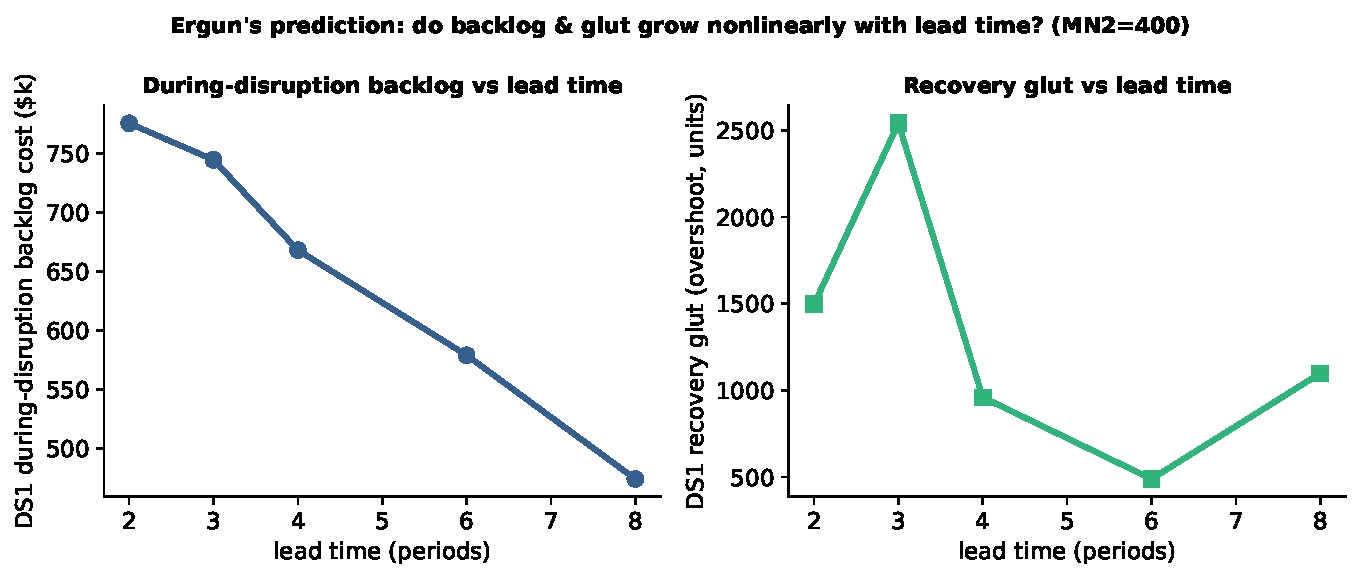
\includegraphics[width=0.86\textwidth]{figures/lt_fig2_cost_vs_leadtime.pdf}
\caption{Ergun's cost prediction, tested. DS1 during-disruption backlog \emph{falls} with lead
time (left; base stock holds a bigger buffer), and the recovery glut is non-monotonic (right) ---
neither grows as predicted.}
\label{fig:ltcost}
\end{figure}

\begin{figure}[h]\centering
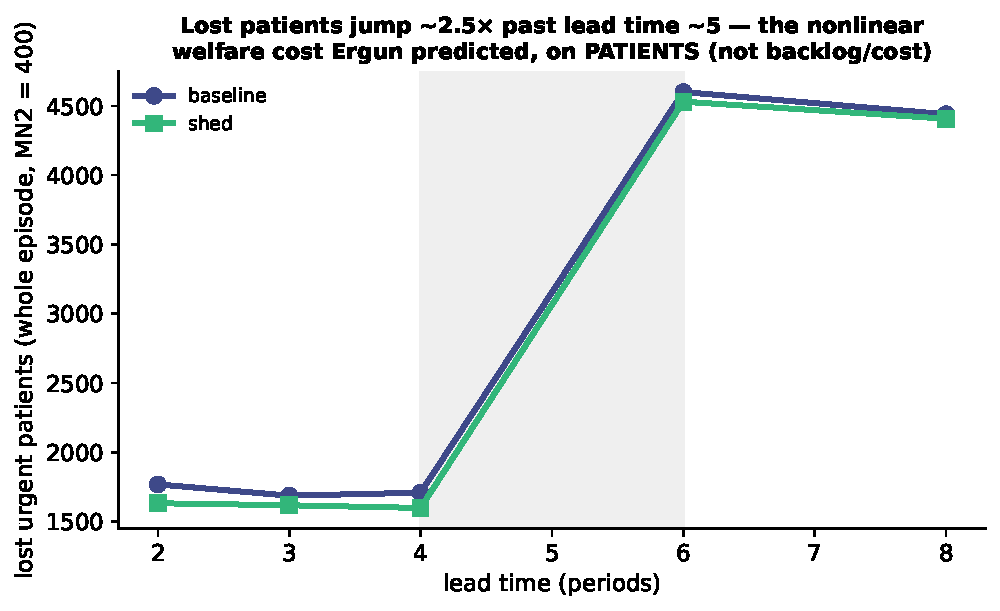
\includegraphics[width=0.74\textwidth]{figures/lt_fig2b_lost_vs_leadtime.pdf}
\caption{Where the nonlinearity is: lost urgent patients (urgent20, MN2 = 400) jump $\sim$2.5$\times$
between lead time 4 and 6. The welfare cost Ergun predicted appears on patients, not cost.}
\label{fig:ltlost}
\end{figure}

\textbf{3. The capacity-flip threshold moves \emph{down}, and the collapse \emph{mildens}, as
lead time grows} (Fig.~\ref{fig:ltflip}, Table~\ref{tab:ltflip}). At LT 2 shed turns
system-harmful below MN2 $\approx$192 and the worst cell is $-5.4$M; by LT 8 the threshold has
fallen to $\approx$157 and the worst cell is only $-1.0$M. A longer pipeline spreads the rerouted
surge over more periods, so the healthy chain congests less acutely --- the misaligned-incentive
collapse is \emph{less} severe at longer lead time, not more. The qualitative story is unchanged
(DS1 still gains from shed; the system still flips negative at low capacity), only the boundary
and the magnitude move.

\begin{table}[h]
\centering\small
\caption{Capacity-flip threshold vs.\ lead time (urgent0): system profit $\Delta$ (shed $-$
baseline), \$M, by MN2 capacity. The flip (sign change) moves to lower capacity and the collapse
mildens as lead time grows.}
\label{tab:ltflip}
\begin{tabular}{r r r r r r r}
\toprule
lead time & 400 & 240 & 180 & 140 & 120 & flip cap \\
\midrule
2 & $+0.64$ & $+0.64$ & $-0.15$ & $-5.41$ & $-4.09$ & 192 \\
3 & $+0.60$ & $+0.60$ & $-0.13$ & $-1.55$ & $-4.07$ & 191 \\
4 & $+0.51$ & $+0.51$ & $+0.07$ & $-1.07$ & $-3.41$ & 177 \\
6 & $+0.42$ & $+0.42$ & $+0.26$ & $-0.67$ & $-2.62$ & 169 \\
8 & $+0.28$ & $+0.28$ & $+0.24$ & $-0.19$ & $-1.04$ & 157 \\
\bottomrule
\end{tabular}
\end{table}

\begin{figure}[h]\centering
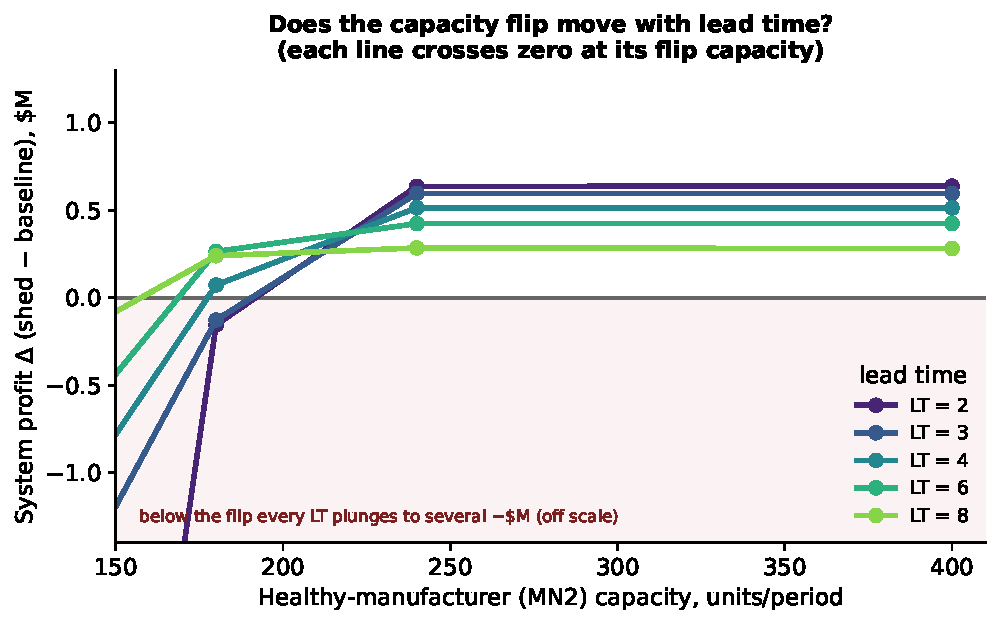
\includegraphics[width=0.78\textwidth]{figures/lt_fig1_flip_vs_leadtime.pdf}
\caption{Capacity-flip threshold vs.\ lead time. Each line is system profit $\Delta$ (shed $-$
baseline) across MN2 capacity at one lead time; it crosses zero at that lead time's flip
capacity. Longer lead time flattens the curve --- less benefit at high capacity, a milder
collapse at low capacity, and a flip that moves \emph{left} (192 $\to$ 157).}
\label{fig:ltflip}
\end{figure}

Floor guard passed at every lead time (no-disruption fill $\approx$1.0 down to MN2 = 120), so the
low-capacity cells are real congestion, not a starved baseline.

\section{Disruption severity $\times$ capacity --- the shed dynamic has a severity threshold}

Sweeping MN1 severity from 35\% to 95\% cut at lead time 2 (Fig.~\ref{fig:sevflip},
Table~\ref{tab:sevflip}) shows that \textbf{the entire shed / capacity-flip phenomenon is a
\emph{severe-disruption} phenomenon.}

\textbf{Below $\sim$65\% cut, shed is completely inert.} System profit $\Delta$ (shed $-$
baseline) is $0.00$ at every capacity, and the disruption barely registers --- system
during-backlog $\approx$1k and lost patients $\approx$33 (versus 2{,}574k and 1{,}768 at 95\%).
At these severities MN1 still produces enough ($\ge$35\% $=\ge$140/period) that, combined with the
base-stock buffer, the disruption is absorbed \emph{without any rerouting} --- so there is nothing
for shed to do, and no misaligned incentive to worry about.

\textbf{The phenomenon switches on at $\sim$80\% cut and intensifies toward 95\%.} At 80\% shed
helps the system ($+0.62$M at high capacity) and the flip appears (system turns negative below
MN2 $\approx$156); at 95\% the flip moves up to $\approx$192 and the collapse deepens to $-5.4$M.
So \emph{more severe $\to$ the flip sits at higher capacity and the collapse is deeper} --- the
misaligned-incentive zone \emph{widens} with severity. This is the severity-dependence Doroudi
et~al.\ flagged: the trust-rerouting dynamic only activates once the disruption is severe enough
to overwhelm the buffer.

\begin{table}[h]
\centering\small
\caption{Capacity-flip vs.\ MN1 severity (LT=2, urgent0): system profit $\Delta$ (shed $-$
baseline), \$M, by MN2 capacity. Shed is inert ($\equiv 0$) below $\sim$65\% cut; the flip
appears and widens above it.}
\label{tab:sevflip}
\begin{tabular}{r r r r r r r}
\toprule
MN1 severity & 400 & 240 & 180 & 140 & 120 & flip cap \\
\midrule
35\% cut & $0.00$ & $0.00$ & $0.00$ & $0.00$ & $0.00$ & --- \\
50\% cut & $0.00$ & $0.00$ & $0.00$ & $0.00$ & $0.00$ & --- \\
65\% cut & $0.00$ & $0.00$ & $0.00$ & $0.00$ & $0.00$ & --- \\
80\% cut & $+0.62$ & $+0.62$ & $+0.62$ & $\mathbf{-0.41}$ & $\mathbf{-2.28}$ & 156 \\
95\% cut & $+0.64$ & $+0.64$ & $\mathbf{-0.15}$ & $\mathbf{-5.41}$ & $\mathbf{-4.09}$ & 192 \\
\bottomrule
\end{tabular}
\end{table}

\textbf{Shed's patient benefit is largest at the activation severity, not the extreme.} At 80\%
cut with abundant capacity, shed nearly \emph{halves} lost urgent patients ($1{,}409\to769$),
because the healthy chain has room to fully serve the rerouted HC1 while residual MN1 production
(20\%) still covers the captive HC2. At 95\% the benefit shrinks ($1{,}768\to1{,}632$) --- with
MN1 nearly dead, even the captive suffers and there is less to gain by rerouting. So the
intervention is most valuable in the band where the disruption is serious but not total.

\begin{figure}[h]\centering
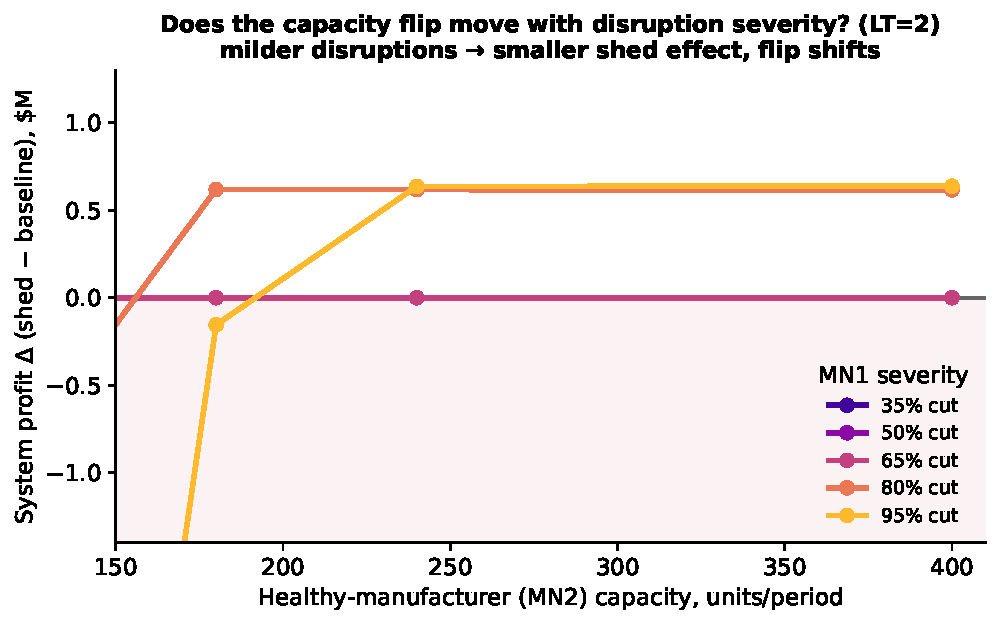
\includegraphics[width=0.78\textwidth]{figures/lt_fig3_flip_vs_severity.pdf}
\caption{Capacity-flip vs.\ MN1 severity (LT=2). Below $\sim$65\% cut shed is flat at zero
(inert, the overlapping lines on the axis); at 80\% and 95\% it activates, and the flip moves to
higher capacity as severity rises --- the misaligned-incentive zone widens with severity.}
\label{fig:sevflip}
\end{figure}

\section*{Pre-registration check and bottom line}

\emph{Predictions vs.\ found.} (1) During-backlog grows with lead time --- \textbf{wrong}, it
\emph{falls} (base stock auto-scales the buffer). (2) Recovery glut grows --- \textbf{wrong}, it
is non-monotonic. (3) Flip threshold moves \emph{up} --- \textbf{wrong}, it moves \emph{down} and
the collapse mildens. (4) Qualitative misaligned-incentive story survives --- \textbf{confirmed}.
(5) Floor risk at long lead time --- \textbf{no breach}. \emph{Unpredicted:} lost patients jump
nonlinearly past lead time $\sim$5.

\medskip
\textbf{Bottom line.} \emph{Lead time:} in a base-stock world, longer lead time does \emph{not}
worsen the distributor's backlog or the misaligned-incentive collapse --- the order-up-to buffer
scales with lead time and absorbs the shock, and a longer pipeline even \emph{softens} the
low-capacity collapse. Ergun's predicted nonlinearity is real but lands on \textbf{patient
welfare}: lost urgent patients jump $\sim$2.5$\times$ once the pipeline exceeds $\sim$5 periods,
and recovery slows. Cost-based metrics understate lead-time risk because base stock hides it as
holding cost; the patient (lost-demand) metric is the one that exposes it.

\emph{Severity:} the shed dynamic and its misaligned-incentive flip are \textbf{gated by
severity} --- they simply do not exist below $\sim$65--80\% cut, where the buffer plus residual
production absorbs the disruption and shed is inert. Above that they switch on and the flip zone
widens toward 95\%. Putting both axes together, the misaligned-incentive collapse is a
\textbf{severe-disruption, scarce-capacity, short-pipeline} phenomenon (worst at 95\% cut /
MN2 $\le$ 180 / lead time 2), while shed is \emph{most valuable} in the serious-but-not-total
band (80\% cut with capacity to absorb the reroute, where it nearly halves lost patients). For
the real world --- where shortages are severe and capacity is scarce --- this says the
distributor's private incentive to shed is exactly where it diverges most from system and patient
welfare.

\end{document}
